\documentclass{article}

% preamble
\usepackage{geometry} 

% encoding
\usepackage[utf8]{inputenc}
\usepackage[T1]{fontenc}

% maths
\usepackage{amstext,amsmath,amssymb}
\DeclareMathOperator{\argmax}{argmax}

% figures, tables
\usepackage[pdftex]{graphicx}
\usepackage{subcaption}
\graphicspath{{Figures/}}
\usepackage{booktabs}
\usepackage{float}

% links
\usepackage[usenames,dvipsnames]{xcolor}
\PassOptionsToPackage{hyphens}{url}\usepackage[
colorlinks=true,
urlcolor=PineGreen,
linkcolor=RoyalBlue,
citecolor=RoyalBlue
]{hyperref}

% bibliography
\usepackage[
backend=biber,
style=authoryear,
citestyle=authoryear,
uniquename=init,
maxcitenames=1,
giveninits=true,
hyperref=auto,
sorting=nyt
]{biblatex}
\addbibresource{references.bib}

% appendix
\usepackage{chngcntr}


% document
\begin{document}

\begin{titlepage}
	\begin{center}
	    % logo
		\begin{figure}[h]
			\centering
			
\includegraphics[width=.25\textwidth]{logo} 
		\end{figure}
		\textsc{Environmental sciences and engineering}\\[0.5cm]
		
		% title
		\newcommand{\HRule}{\rule{\linewidth}{0.2mm}}
		\HRule \\[0.5cm]
		{\large SIE Project}\\[0.2cm]
		{\huge Confidence Estimation for Convolutional Neural\\[.2cm] Networks using Density Trees
		}\\[0.5cm]
		\HRule \\[0.5cm]
		
		% Author and lecturer
		\begin{minipage}[t]{0.45\textwidth}
			\begin{flushleft} \large
				\emph{Author:}\\[0.2cm]
				Cyril \textsc{Wendl}
			\end{flushleft}
		\end{minipage}
		\hfill
		\begin{minipage}[t]{0.45\textwidth}
			\begin{flushright} \large
				\emph{Supervisors:}\\[0.2cm]
				Prof. Devis \textsc{Tuia} (WUR)\\
				Diego \textsc{Marcos} (WUR)\\
				Prof. François \textsc{Golay} (EPFL)\\
				Fall semester 2017
			\end{flushright}
		\end{minipage}
		\vfill
		
		{\large Lausanne, \today}
	\end{center}
\end{titlepage}

\section{Introduction}
Convolutional Neural Networks (CNN) have become a crucial tool for image recognition in a wide range of domains including bio-medical applications or automatic land use classification using satellite imagery to name just a few (\cite{Volpi2017DenseSL,kampffmeyer, ucf}). The ability of Convolutional Neural Networks to recognize the context, structure and underlying features of images has led to numerous new applications.\\

While CNN have superseded many supervised classification approaches in terms of accuracy, much research still goes into the estimation of the uncertainty associated with the classification result. These are not naturally provided by CNN models. In supervised classification approaches it is desirable that whenever a new class is introduced in a prediction sample which has not been seen during training, a low confidence tells the user to manually check the classification result, which is crucial in many domains. A reliable assessment of the uncertainty of a model is also crucial in many environmental tasks such as remote sensing, including tasks such as land use classification and change detection after natural disasters (\cite{menderes_automatic_2015, womble_automated_2007, postadjian_investigating_2017}). All of these domains could benefit from having better uncertainty indicators. Much research has already gone into the topic of providing accuracy measures in CNN models. For instance, \cite{ghahramani} have tried to model uncertainty in deep learning averaging dropout of predictions on the test set as an approximation of Bayesian uncertainty while \cite{subramanya} have tried to take uncertainty into account using density modelling, which does not rely on the Softmax activation function.\\


% Objective
This study presents an uncertainty estimation approach based on density clustering of the activation layer of the fully-connected layer in a Convolutional Neural Net, applying this method to the MNIST dataset (\cite{mnist}). The activation weights are retrieved during inference and are clustered using a density Tree to predict the probability of the activation weights of each image to belong to one of the clusters. Similar to random forests, which use many decision trees to separate labelled data, density forests separate unlabelled data using several density trees. An Information Gain function is used to determine the best data splits in each tree by maximizing the Gaussianity within each data cluster. Unlike decision trees, the goal of density trees is not to predict a label but to best partition the data into homogeneous clusters. Density forests can be compared to Gaussian Mixture Models (GMM) or \textit{k-means} (\cite{decisionForests-MSR}), which are common clustering methods used for unlabelled data.\\

% Prediction
For a given data point, each of the trained density trees is descended until the leaf node and the probability of the point to belong to this cluster is calculated. The mean of these probabilities over all trees is used as an uncertainty measure for the given point. The hypothesis is that points belonging to a class seen during training of the CNN will be more likely to belong to one of the clusters than a point belonging to an unseen class. The relative difference between the uncertainty of several points can be used to detect irregularities. This uncertainty method is compared to a baseline method, consisting of the margin between the predicted membership probability of the most likely class and the second most likely class.


\section{Methodology}

% Decision Trees
\subsection{Decision Trees}
A decision tree is a binary tree consisting of hierarchical nodes and edges which, at each level, provides the most important features to determine the outcome of a dependent variable, given an arbitrary number of independent variables (\cite{decisionForests-MSR}). At each level starting from top to bottom, the goal of a Decision Tree is to find the best possible split to partition the feature space such as to minimize the entropy in every subdomain. A decision tree can grown until there is exactly one class label at each leaf node, or it can be stopped before.\\

The following notation is based on \cite{decisionForests-MSR}. Vectors are denoted in bold ($\boldsymbol{v}$), matrices in telescope uppercase letters ($\mathtt{M}$) and sets using calligraphic notation ($\mathcal{S}$). Furthermore, following notation is used for classes and membership probabilities:
\begin{align}
\mathcal{L}&=\{c_i\}_{1\leq i\leq n_c}&& \text{Set of classes}\\
P^{(c)}(x)&=P(x\in c)&& \text{Membership probability of a sample x to class c}
\end{align}

At every splitting step, an Information Gain function is maximized:

\begin{equation}
    \label{eq:ig}
    I = H(\mathcal{S})-\sum_{i\in \{1,2\}}\frac{|\mathcal{S}^i|}{|\mathcal{S}|}H(\mathcal{S}^i)
\end{equation}

As an optimizer function, the Shannon entropy has been used:
\begin{equation}
    H(\mathcal{S}) = -\sum_{c\in\mathcal{C}}P^{(c)}\log(P^{(c)})
\end{equation}

That is, for every class and every possible split, it is checked whether the entropy is minimized, i.e., whether the information gain is maximized. Searching of the optimal split value has been performed on a regular grid between the minimum and maximum of all data points, i.e.,  for every dimension, an array of possible values linearly spaced between the minimum and maximum data values were considered as possible splitting candidates.\\

The implemented data structure of a decision tree node is represented in appendix \ref{subsec:implementation}.\\

A first, naïve approach consists of splitting a single decision tree until there is only one type of leaf node left in each leaf node, leading to  strong overfitting and noisy decision boundaries. A more sophisticated approach consists in combining several decision trees.

% Random Forests
\subsection{Random Forests}
 More smooth and generalized boundaries can be obtained by using Random Forests, which combine a set of individually trained trees on random subsets of the initial data (\cite{decisionForests-MSR, Breiman2001}). In this study, a simple implementation of Random Forests is provided, training multiple decision trees in parallel on different, random subsamples of the dataset.\\

% Density forests
\subsection{Density Forests}
The methods explained above only work for labelled data. In order to determine to which subspace an unlabelled data point belongs, clustering methods such as \textit{k-means}, Gaussian mixture models (GMM) or density forests can be used. density trees aim at modelling the underlying distribution that has generated some data. Similar to decision trees, information gain is used to determine the best split at each level of the density tree. The generic information gain formula to be maximized is the same as the one used for decision trees (eq. \ref{eq:ig}). An unsupervised entropy function is designed based on the assumption of a multivariate Gaussian distribution at each tree node to find the split that maximizes Gaussianity both split sides of the node (\cite{decisionForests-MSR}):
\begin{equation}
    H(\mathcal{S}) = \frac{1}{2}\log\Big((2\pi e)^d|\mathtt{\Lambda}(\mathcal{S})|\Big)
\end{equation}
$\mathtt{\Lambda}$ being the associated $d \times d$ covariance matrix. Hence, the information gain at the $j^{\text{th}}$ split becomes (\cite{decisionForests-MSR}):
\begin{equation}
    I_j = \log(|\mathtt{\Lambda}(\mathcal{S}_j)|) - \sum_{i\in \{L, R\}}\frac{|\mathcal{S}_j^i|}{|\mathcal{S}_j|}\log(|\mathtt{\Lambda}(\mathcal{S}_j)|)
\end{equation}

For a description of the motivation behind this optimization method, refer to \cite{decisionForests-MSR}. The implemented data structure for density trees is represented in in appendix \ref{subsec:implementation}.\\

At prediction time, a given data point descends the density tree according to the split dimension and value associated with each tree node until it reaches a leaf node. The probability of the data point to belong to a cluster of the tree is calculated with respect the leaf node cluster (\cite{decisionForests-MSR}):
\begin{equation}
    \label{eq:proba_density}
    p_t(\boldsymbol{x}) = \frac{\pi_l}{Z_t}\mathcal{N}(\boldsymbol{x}|\boldsymbol{\mu}_{l(\boldsymbol{x})},\mathtt{\Lambda}_{l(\boldsymbol{x})})
\end{equation}
With $\boldsymbol{\mu}_{l(\boldsymbol{x})}$ and $\mathtt{\Lambda}_{l(\boldsymbol{x})}$ denoting the mean and covariance of the leaf node corresponding to the data point $\boldsymbol{x}$, $\pi_l$ being the proportion of points falling into the respective leaf node and $Z_t$ a partition function ensuring normalization of the data. The multivariate Gaussian distribution is defined as follows:
\begin{equation}
    \mathcal{N}(\boldsymbol{x}|\boldsymbol{\mu},\mathtt{\Lambda})=\frac{1}{\sqrt{(2\pi)^k\det\mathtt{\Lambda}}}\exp\Big({-\frac{1}{2}(\boldsymbol{x}-\boldsymbol{\mu}})^\top\mathtt{\Lambda}^{-1}(\boldsymbol{x}-\boldsymbol{\mu})\Big)
\end{equation}

Where $\boldsymbol{\mu}$ is the mean, $\mathtt{\Lambda}$ is the co-variance matrix and $k$ is the number of dimensions of $\boldsymbol{x}$ (\cite{scipy}). The thus obtained probability is weighted by the percentage $\pi_l$ of all the data used for training the density tree falling into this leaf node. For the purpose of this study, a simple density forest without the probability normalization term $Z_t$ was implemented. However, for comparisons between several models, the output probabilities would need to be normalized by a partition function $Z_t$ as in equation \ref{eq:proba_density}.\\

At every step of the density tree creation, splits are created such as to maximize the Gaussianity on both sides of the node. The density tree continues splitting the node having the biggest entropy at each step of building the tree. The maximum number of splits can either be based on an Gaussianity criterion, maximum tree depth or be fixed to an arbitrary number. On the synthetic data set presented below the number of splits was fixed.\\

\subsection{Data Generation}
In order to study the behaviour of the implemented methods, some dummy data has been generated according to Gaussian distributions. All methods have been tested with data generated in higher-dimensional space, however visual results are presented for two-dimensional data. The Data has been generated according to the following method:\\

First, a number of clusters is defined. For each cluster, a given number of points is generated based on Gaussian multivariate distribution, using a predefined covariance and a random mean within a pre-defined interval. For each cluster, the covariance is arbitrarily increased and decreased along certain dimensions. The generated points of some arbitrarily selected clusters are sheared and shifted to produce non-linear data distributions. An example of such generated data is given in figure \ref{fig:gen-data}.


\begin{figure}[H]
    \begin{subfigure}{0.49\textwidth}
        \centering
        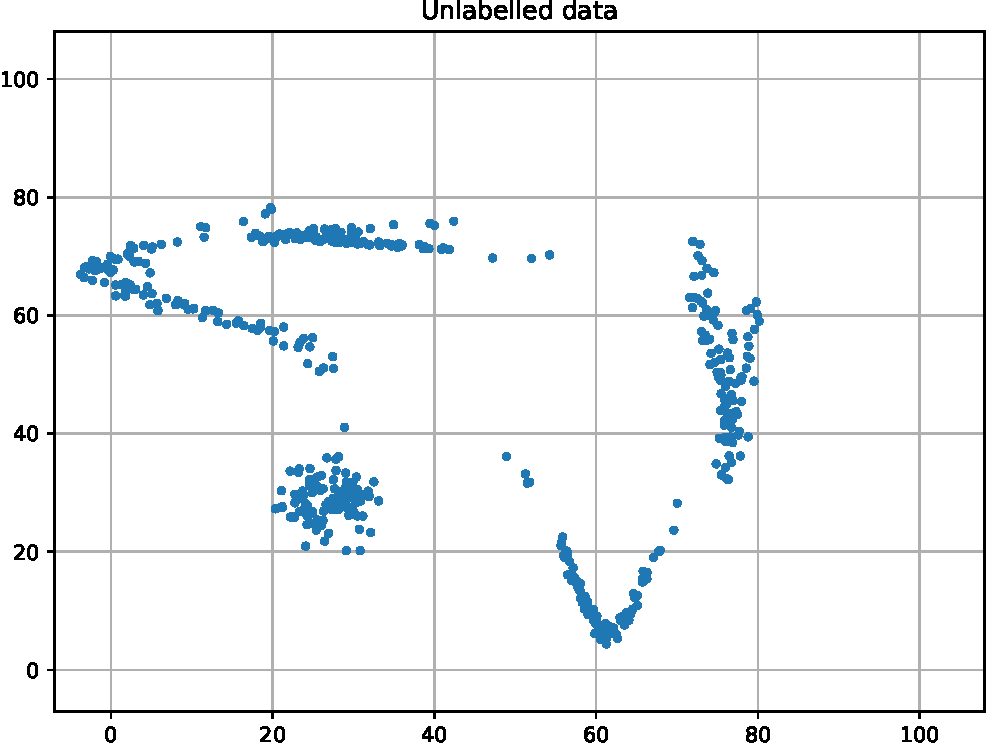
\includegraphics[width=\textwidth]{unlabelled-data.pdf}
        \caption{Unlabelled Data in 5 clusters}
        \label{subfig:unlabelled-data}
    \end{subfigure}
    \begin{subfigure}{0.49\textwidth}
        \centering
        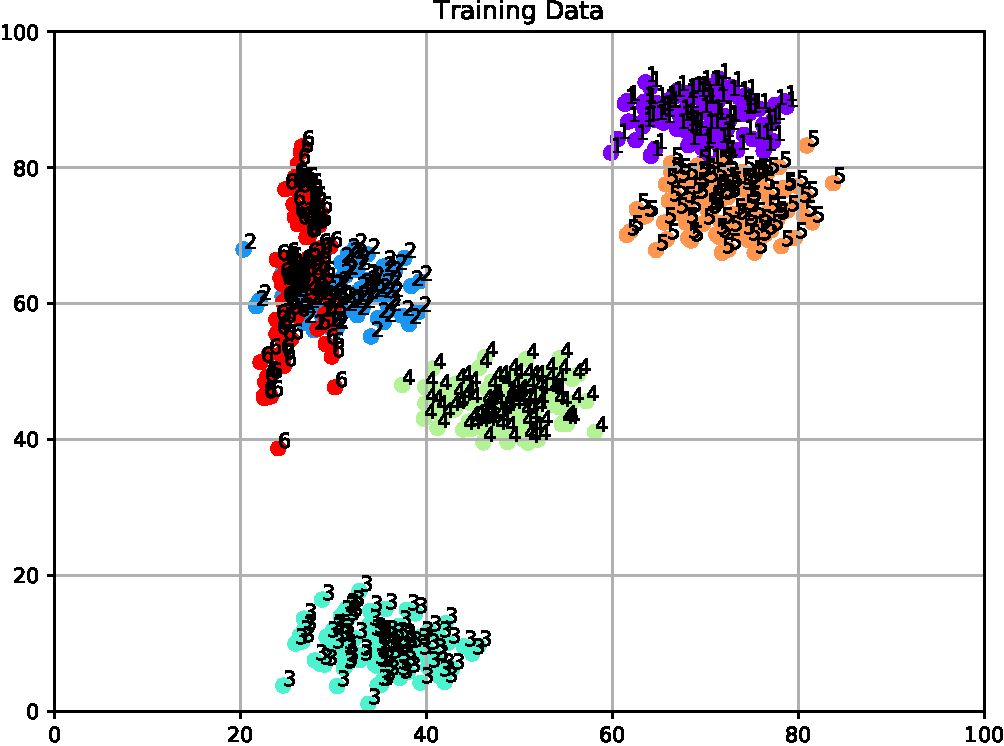
\includegraphics[width=\textwidth]{labelled-data.pdf}
        \caption{Labelled Data in 6 clusters}
        \label{subfig:labelled-data}
    \end{subfigure}
    \caption{Randomly generated labeled and unlabelled Data for the task of classification by a Random Forest model and clustering by density forest respectively. Clusters are indicated by the point color and the corresponding cluster label.}
    \label{fig:gen-data}
\end{figure}

% Application to MNIST
\subsection{Application to the MNIST Dataset}
% CNN Architecture
In addition to the generated dummy data, a Convolutional Neural Network has been trained on the MNIST Dataset (\cite{mnist}). Dropout was performed to increase the redundancy of the network and avoid overfitting. The ReLU activation function ($f(x) = max(0, x)$) was used in each layer of the network. The full architecture is described in table \ref{table:CNNArchitecture}.

% Table showing the architecture
\begin{table}[H]
    \begin{center}
    \begin{tabular}{ll}
    \toprule
    Type & Remarks \\
    \hline
    Input & Dimension $n_{batch} \times 28 \times 28$ \\ 
    Convolution + ReLU & 32 3 $\times$ 3 filters\\
    Convolution + ReLU & 64 3 $\times$ 3 filters\\
    MaxPooling & 2 $\times$ 2 pool size \\
    Dropout & Dropout Factor = 0.25 \\
    \hline
    Flatten & \\
    Dense (FC) + ReLU & 128 neurons\\
    Dropout & Dropout Factor = 0.5 \\
    Output + Softmax & 9 neurons \\
    \bottomrule
    \end{tabular}
    \caption{Architecture of the CNN used for MNIST digit classification.}
    \label{table:CNNArchitecture}
    \end{center}
\end{table}


The activation weights at inference time were retrieved and fed to the density tree. Since the Fully Connected layer contains 128 filters, for a batch $n$ images, the activation weights retrieved during prediction are of dimension $n\times 128$ and contain a lot of redundancy, which causes matrix inversion issues during the calculation of the Gaussian entropy. Therefore, a dimensionality reduction was performed using Principal Component Analysis (PCA), keeping the 30 first dimensions, which were found to explain over 95\% of the variance of the original data (fig. \ref{fig:pca_components}).\\

\begin{figure}[H]
    \centering
    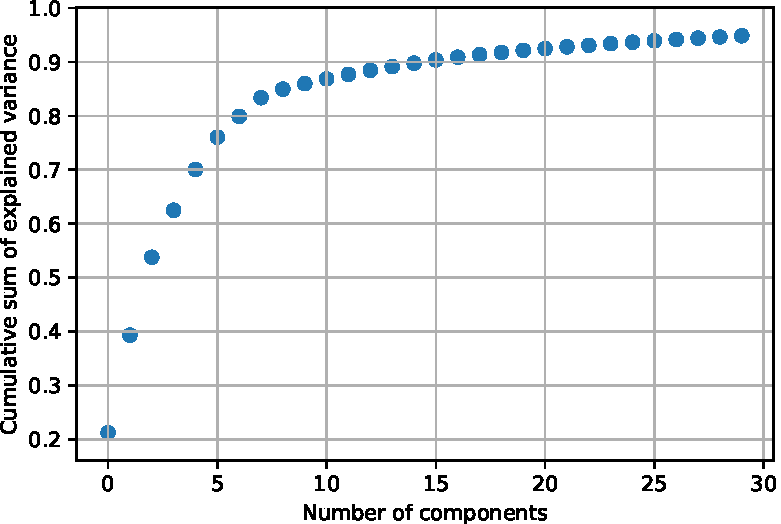
\includegraphics[width=.5\textwidth]{pca_components}
    \caption{Explained variance as a function of the number of components}
    \label{fig:pca_components}
\end{figure}

Although the first three components only explain 54 \% of the variation of the original data, the clusters are already recognizable (fig. \ref{fig:pca_components_3d}).\\

\begin{figure}[H]
    \centering
    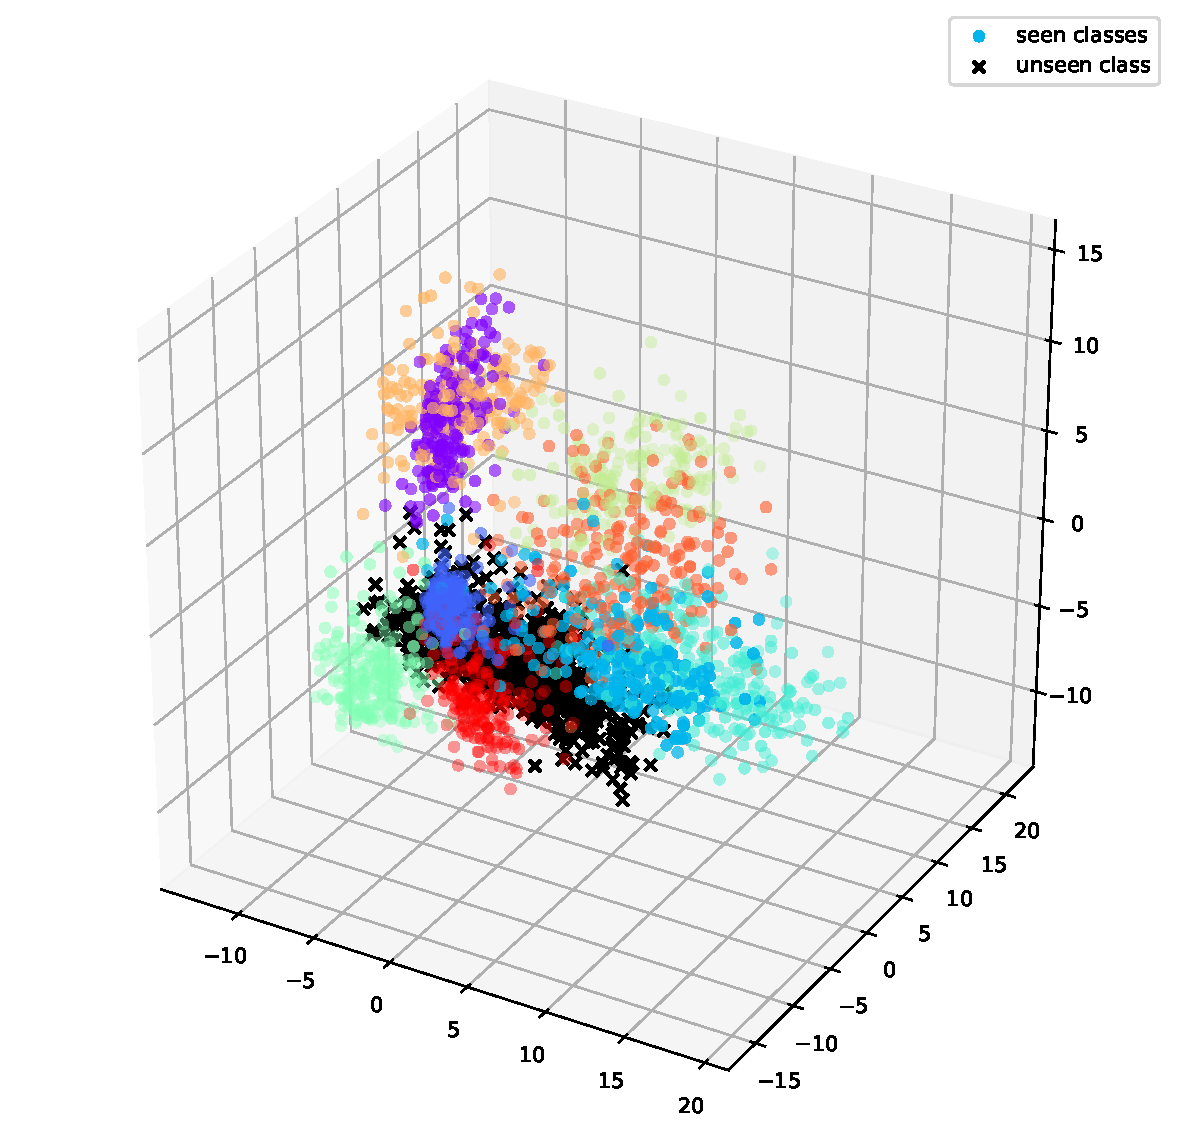
\includegraphics[width=.7\textwidth]{pca_components_3d}
    \caption{First three PCA components colored by class label of the data points, explaining 54\% of the variance of the original data. The unseen class is indicated with black crosses.}
    \label{fig:pca_components_3d}
\end{figure}

The CNN was trained on 53735 samples of images of all classes except one class and validated on 8972 samples, which corresponds roughly to a 85 / 15 split of training and testing data. The class left out in the presented results was the one containing the images of the digit "7".\\

The class membership probabilities obtained during the prediction are compared between both the seen classes and the unseen class. The certitude of the model is assessed as the margin between the highest class probability and the second highest probability (\cite{ouerghemmi_two-step_2017}):

\begin{equation}
    margin(x)=P^{(cbest1)}(x)-P^{(cbest2)}(x)
\end{equation}
where $x$ a given data point, $cbest1=\argmax_{c\in\mathcal{L}}P^{(c)}(x)$ and $cbest2=\argmax_{c\in\mathcal{L}\setminus cbest1}P^{(c)}(x)$. The class membership probability margins of both the seen and unseen images are compared using a ratio, which serves as a baseline for comparing uncertainty measures.\\

A density tree is created on the dimensionality-reduced activation weights of the fully connected layer of the CNN trained on 9 classes. The mean Gaussian probability of each data point to belong to the leaf nodes of the density tree is compared between all seen and unseen classes.

\section{Results}



\subsection{Labelled Data}
% density trees on Randomly generated data
The results of the decision tree applied to Dummy Data are shown in figure \ref{fig:decision-boundaries}. The ruggedness of the decision boundaries is in part due to visualizing the decision boundaries on a discrete mesh of values.

\begin{figure}[H]
    \centering
    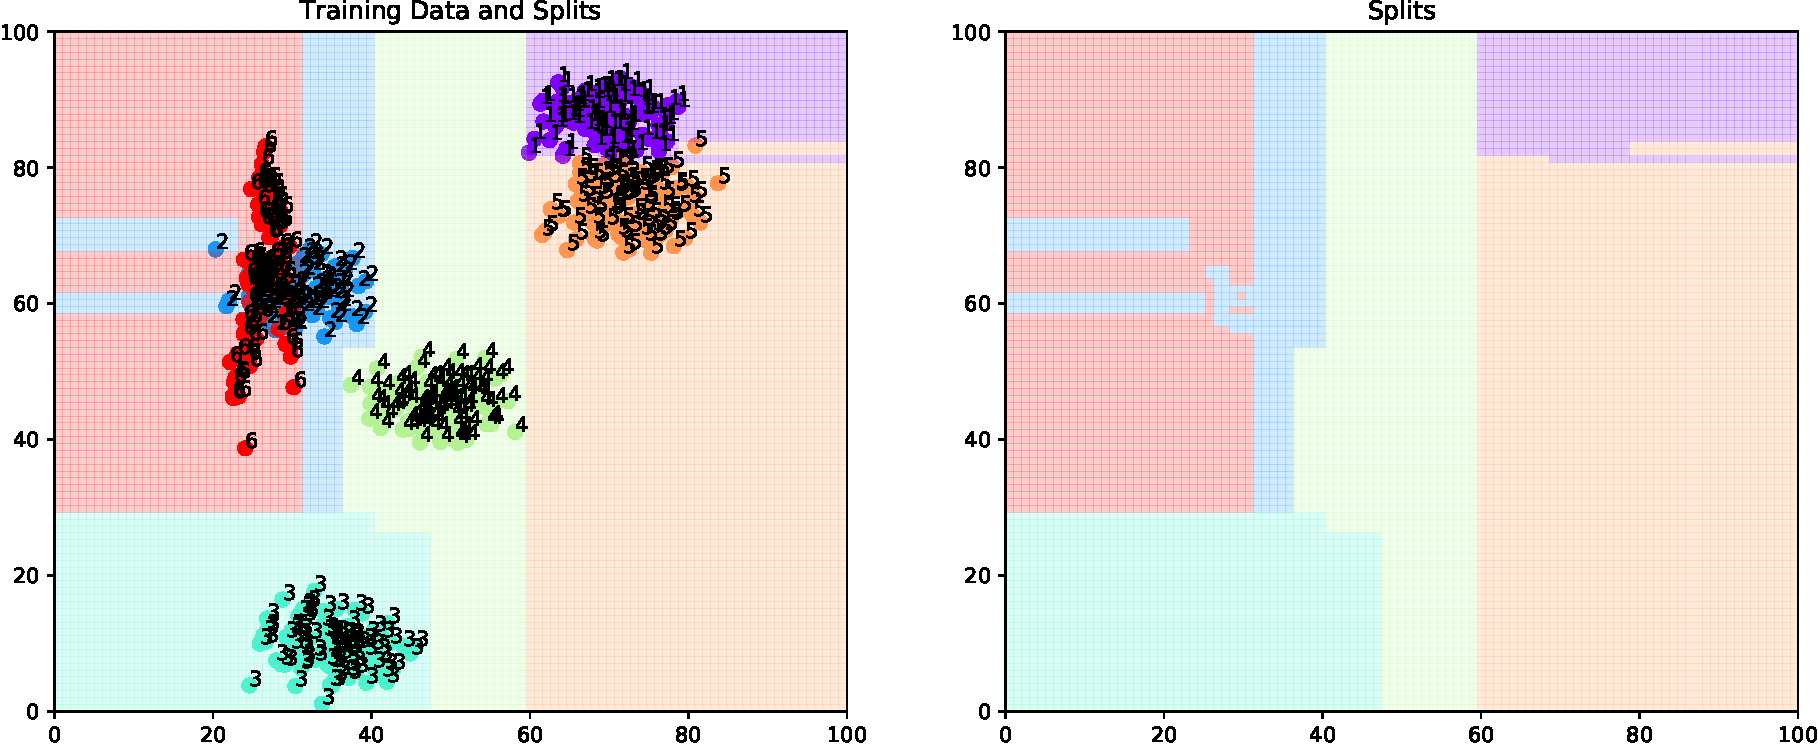
\includegraphics[width=\textwidth]{decision_boundaries.pdf}
    \caption{Decision Boundaries of a single decision tree on 2-dimensional dummy data, splitting the data until every leaf node only contains data of one cluster. Left: decision boundaries with Data, right: decision boundaries only. The decision tree clearly overfits the data.}
    \label{fig:decision-boundaries}
\end{figure}
The decision tree with unlimited depth clearly overfits the data and tends to produce edgy boundaries. The associated decision tree is shown in figure \ref{fig:decision_tree}.

\begin{figure}[H]
    \centering
    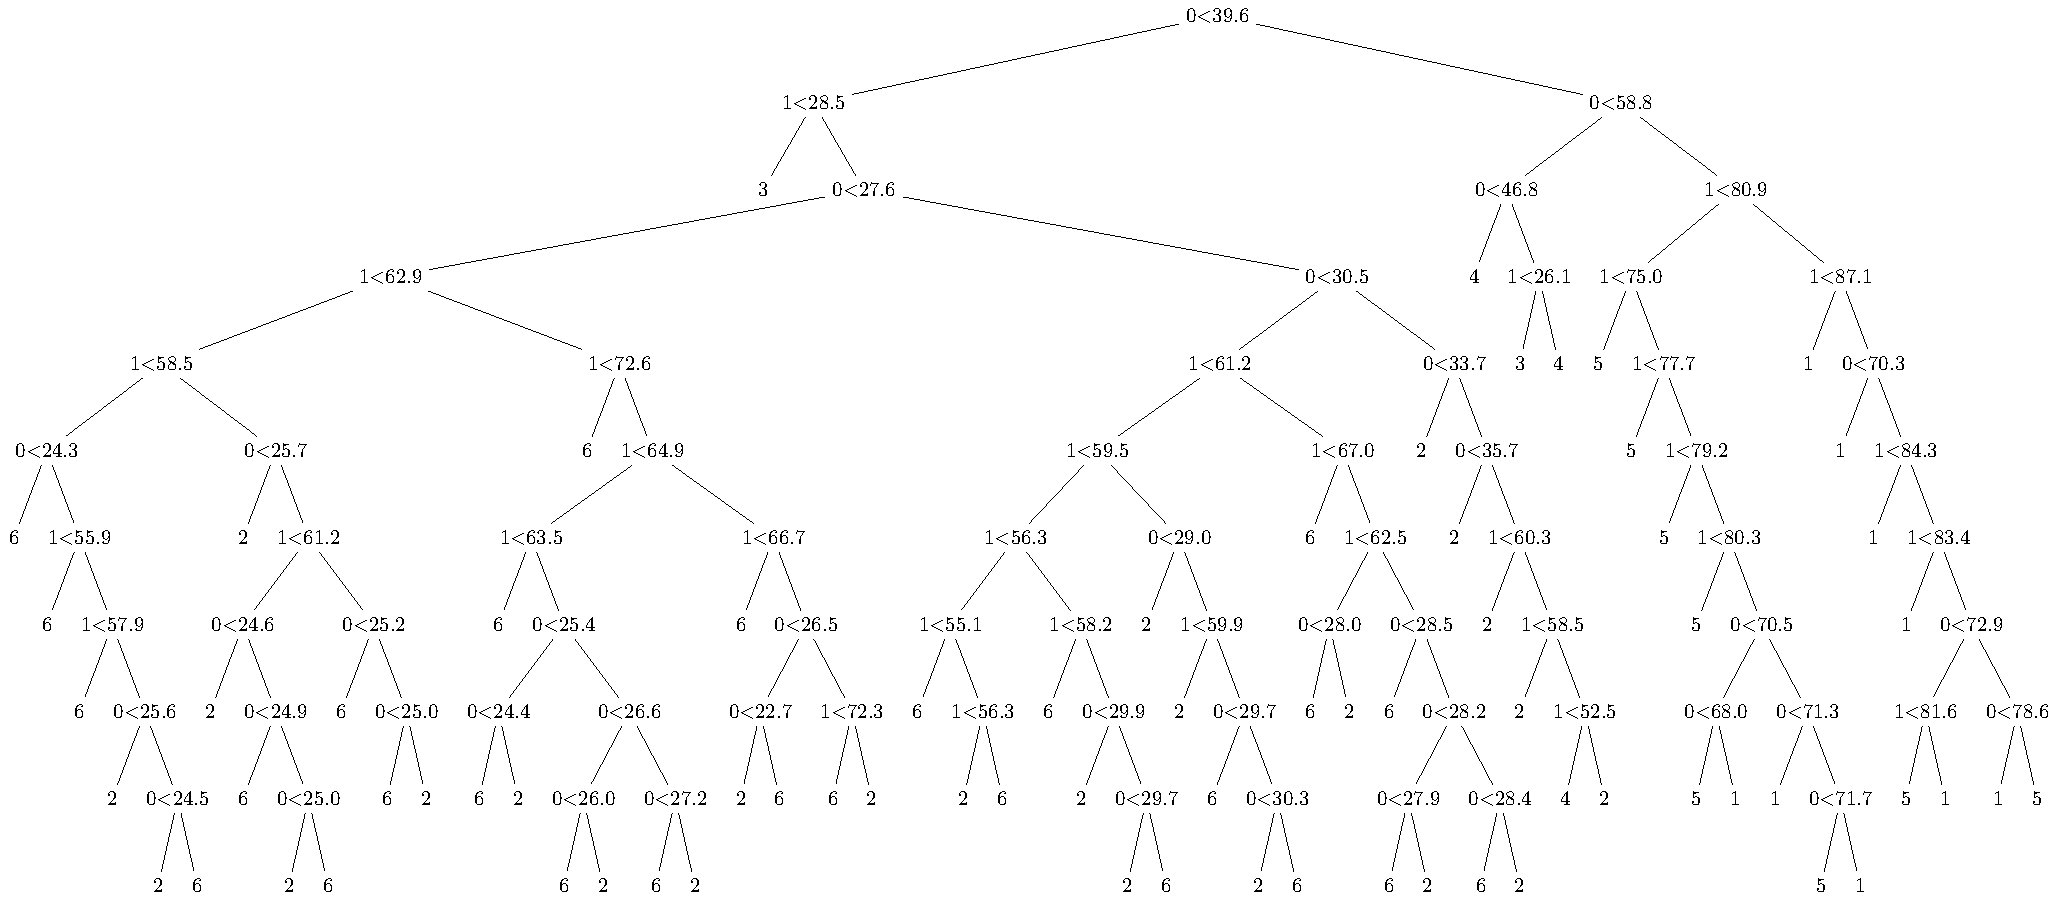
\includegraphics[width=\textwidth]{decision_tree.pdf}
    \caption{Decision tree with unlimited depth on the training data for shown for illustrative purposes, with the split dimension and value at every non-leaf node and the class label at every leaf node. The tree clearly overfits the data and produces edgy decision boundaries}
    \label{fig:decision_tree}
\end{figure}


The classification using Random Forests is shown in figure \ref{fig:rf}.

\begin{figure}[H]
    \centering
    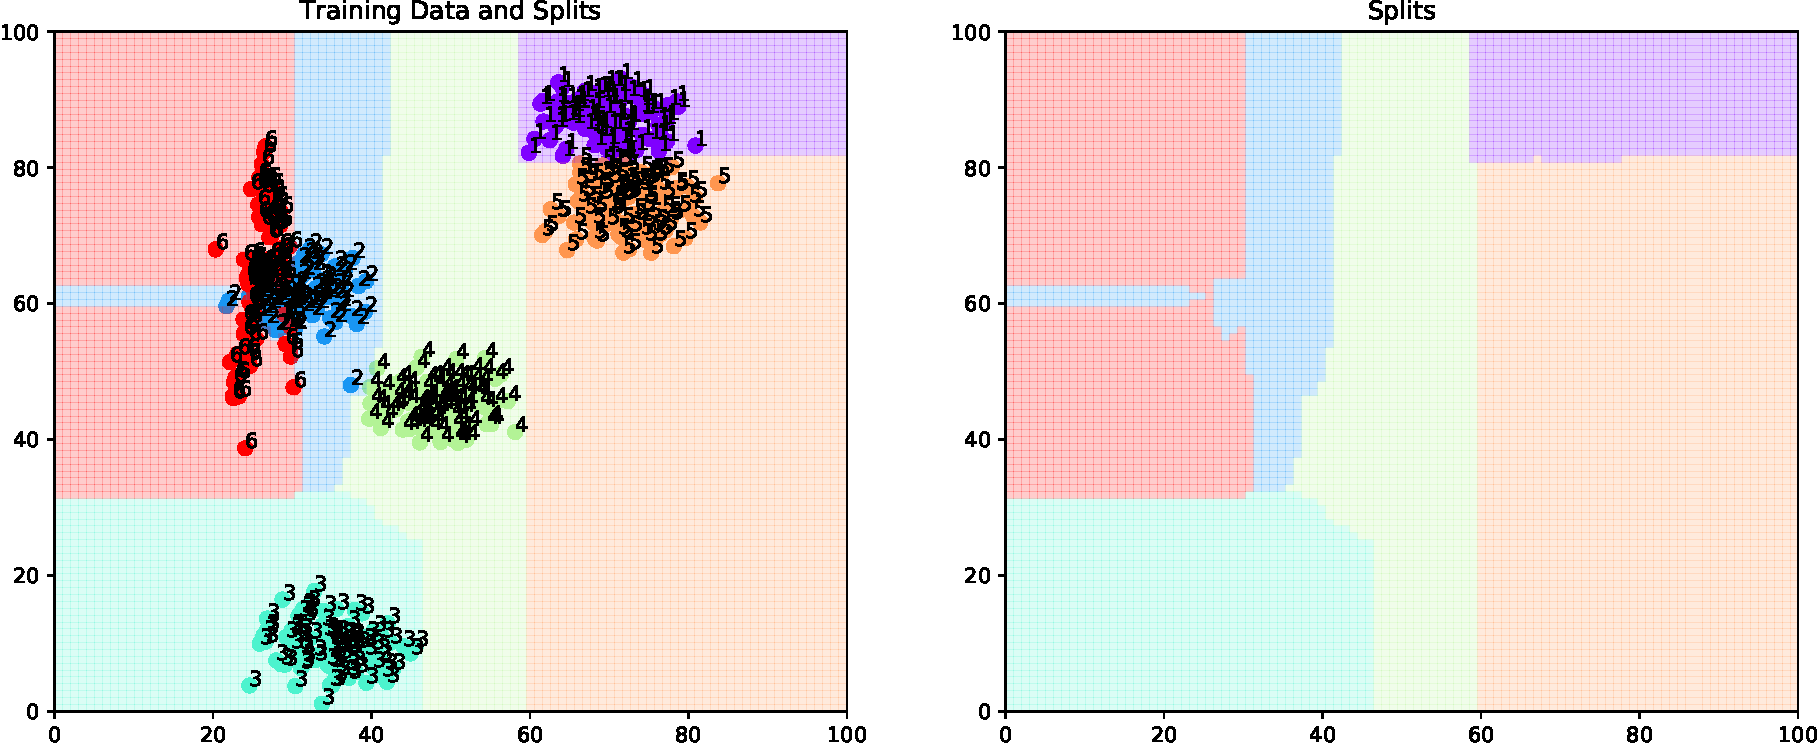
\includegraphics[width=\textwidth]{rf}
    \caption{Decision Boundaries of a Random Forest on 2-dimensional dummy data. 1000 decision trees have been trained on a 30\% random subsample of the original data. Left: decision boundaries with Data, right: decision boundaries only. The Random Forest manages to smooth  out the class decision boundaries.}
    \label{fig:rf}
\end{figure}

\subsection{Unlabelled Data}
% density tree on Unlabelled Dummy Data
The result of applying a single density tree with a total of 4 splits (number of clusters - 1) to the generated dummy data of figure \ref{subfig:unlabelled-data} is shown in figure \ref{fig:unlabelled-data-cov}.

\begin{figure}[H]
    \centering
    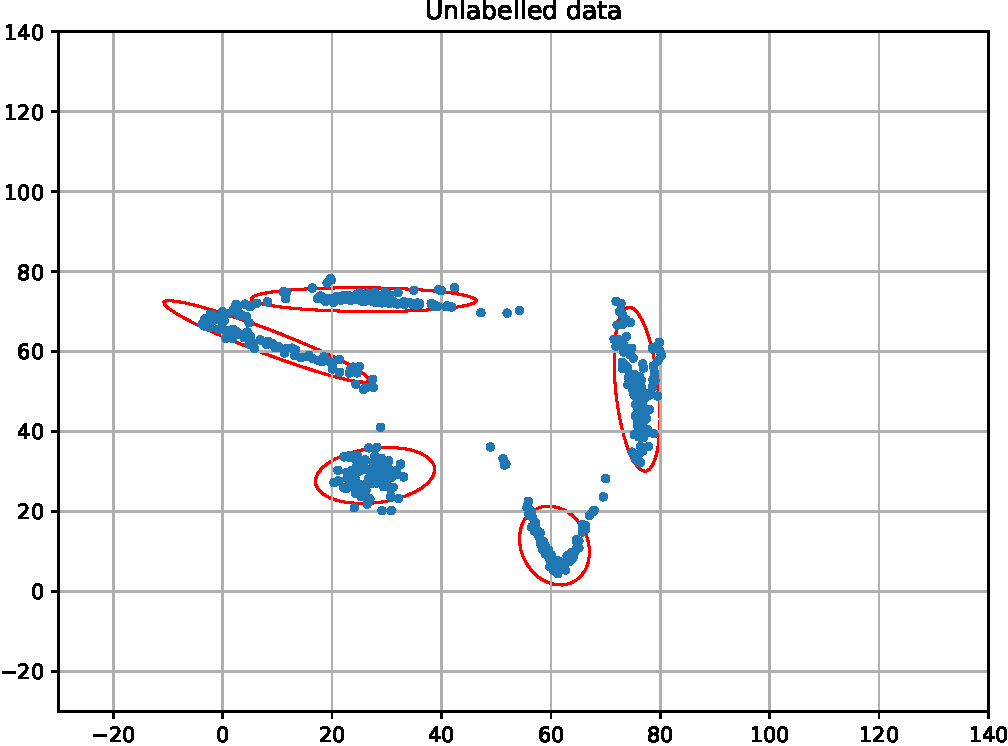
\includegraphics[width=.7\textwidth]{unlabelled-data-cov.pdf}
    \caption{Unlabelled dummy data and covariance ellipses of the density tree leaf nodes.}
    \label{fig:unlabelled-data-cov}
\end{figure}

The splits associated with the density tree are shown in figure \ref{fig:density-tree}.

\begin{figure}[H]
    \centering
    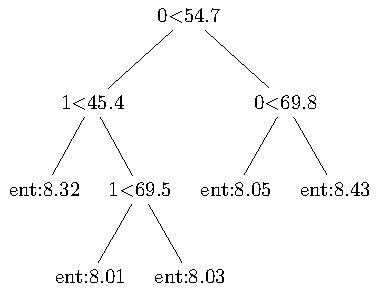
\includegraphics[width=.45\textwidth]{density-tree.pdf}
    \caption{Density tree produced on the training data, with a maximum number of splits set to 4 (number of clusters -1). At every level of the tree, the split dimension and the split value are indicated, and the leaf nodes contain the Gaussian entropy value of the corresponding cluster.}
    \label{fig:density-tree}
\end{figure}


\subsection{MNIST Dataset}
The CNN was trained on 53735 training samples and validated on 8972 samples according to the CNN architecture in table \ref{table:CNNArchitecture}, yielding a validation accuracy of over 99\% after just 5 epochs.\\

When predicting the labels for the unseen class 7, 9 and 3 were the labels most often predicted (fig \ref{fig:pred-count}). Obviously, the label 7 was never predicted since it was unknown to the model.


\begin{figure}[H]
    \centering
    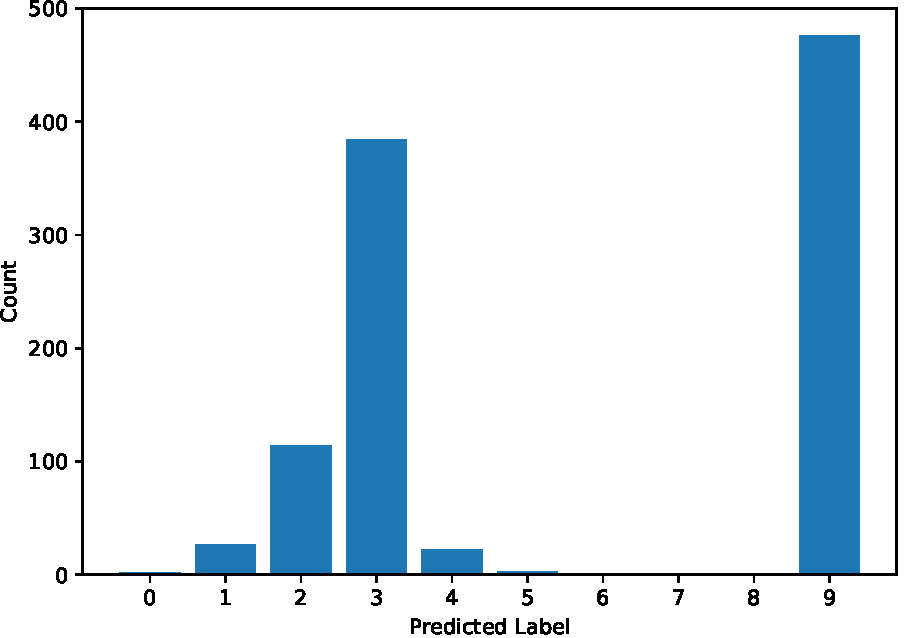
\includegraphics[width=.7\textwidth]{pred-count.pdf}
    \caption{Class predictions for the unseen class 7}
    \label{fig:pred-count}
\end{figure}

Baseline accuracy measures for the prediction on images of seen classes and images of the unseen class are given in table \ref{table:baseline-accuracy}.

\begin{table}[H]
    \centering
    \begin{tabular}{lll}\toprule
    Indicator & Seen class labels & Unseen class label \\\hline
    Margin average & 98.85 \% & 70.07 \% \\
    Margin std & 7.22  \% & 30.46 \% \\
    Predictions $>$ 95 \% & 96.59 \% & 30.93 \%
    \\ \bottomrule
    \end{tabular}
    \caption{Baseline accuracy indicators for predictions on images of the seen class labels and images of the unseen class label.}
    \label{table:baseline-accuracy}
\end{table}

A clear overestimation of the certainty for the unseen label can be observed, with an average margin of 70.07 \% between the probability of the most likely class and the second most likely class. Over 30 \% of all predictions on the unseen class are made with a certitude of over 95 \%.\\

In order to improve on these indicators, a density forest has been built on the activation weights of the seen classes during prediction. The average probability of a label to belong to the cluster of the leaf node of all trees in the density forest trained on 500 individual density trees is summarized in table \ref{table:density-forest-accuracy}. 

\begin{table}[H]
    \centering
    \begin{tabular}{lll}\toprule
    Indicator & Seen class labels & Unseen class label \\\hline
    Mean certainty measure [$\times 1e+22$] & 477.93 & 9.61\\
    Std of certainty measure [$\times 1e+22$] & 1955.62 & 53.85 \\
    \\ \bottomrule
    \end{tabular}
    \caption{density forest Uncertainty measures}
    \label{table:density-forest-accuracy}
\end{table}

The uncertainty ratio between the seen and the unseen class is now 49.74 and reflects to a greater degree the uncertainty of the model.

\section{Conclusion}
% RF, density forests
Random Forests and density forests are powerful tools to cluster data. Satisfying results have been achieved implementing and applying Random Forests to labelled data and density forests to unlabelled data. The application of density trees to dummy data shows its capability to detect clusters in an unsupervised fashion and can be used to provide a more reliable uncertainty measure of a CNN class label prediction.\\

% MNIST
The application to the MNIST dataset clearly shows an overestimation of the certitude by the CNN model, with over 30\% of labels of an unseen class being labelled with a certitude above 95 \%. The average certitude between predictions on images of seen classes and predictions on images of the unseen class differs by less than a factor 2. Using the density forest estimation at test time, a much larger ratio of a factor of 20-30 is observed between the confidence assigned to seen classes with respect to the unseen class. However, the assessment of activation weights during prediction involves the assumption to hold true that the number of classes is really known in advance requires the training set to be "pure". More testing needs to be done to see if the uncertainty measure can also be applied to other, more challenging situations, such as training of impure classes containing mixed labels. Furthermore, more complex case studies need to be assessed, such as land use classification using multi-spectral data. Nevertheless, this study offers an interesting \textit{a posteriori} starting point for improving on the uncertainty measure of Convolutional Neural Networks.

\newpage
\printbibliography



\newpage
\renewcommand{\thesubsection}{\Alph{subsection}}
\counterwithin{figure}{subsection}
\counterwithin{table}{subsection}
\pagebreak  

\section{Appendices}
\subsection{Implementation}
\label{subsec:implementation}
Implementation of all the methods is provided on GitHub: \url{https://github.com/CyrilWendl/SIE-Project}. Several individual Jupyter notebooks are provided to illustrate the steps to produce the \href{https://github.com/CyrilWendl/SIE-Project/blob/master/Code/decision_tree.ipynb}{Decision tree and random forest}, \href{https://github.com/CyrilWendl/SIE-Project/blob/master/Code/density_tree.ipynb}{Density trees} and CNN on the \href{https://github.com/CyrilWendl/SIE-Project/blob/master/Code/MNIST.ipynb}{MNIST dataset}.

\begin{figure}[H]
    \centering
    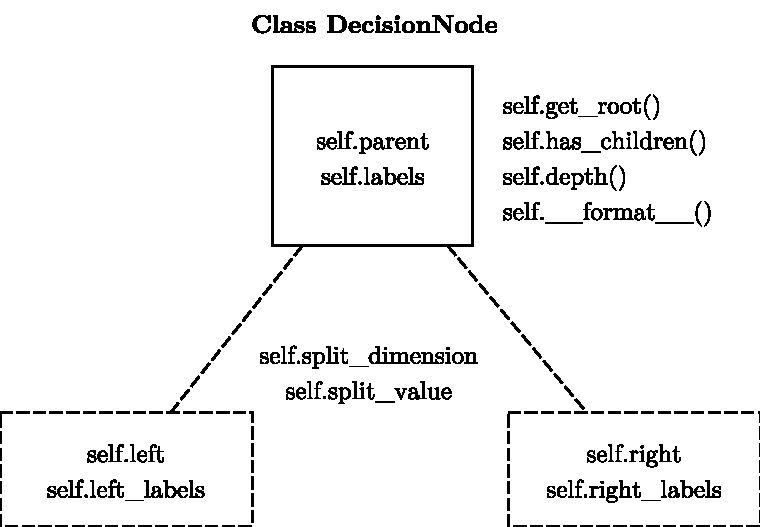
\includegraphics[width=.4\textwidth]{decision-node.pdf}
    \caption{Implemented data structure for decision tree nodes. Every node saves a pointer to its parent, the unique labels contained at its split level, the split dimension and value, methods for traversal and formatting as well information about its child nodes.}
    \label{fig:decision-node}
\end{figure}

\begin{figure}[H]
    \centering
    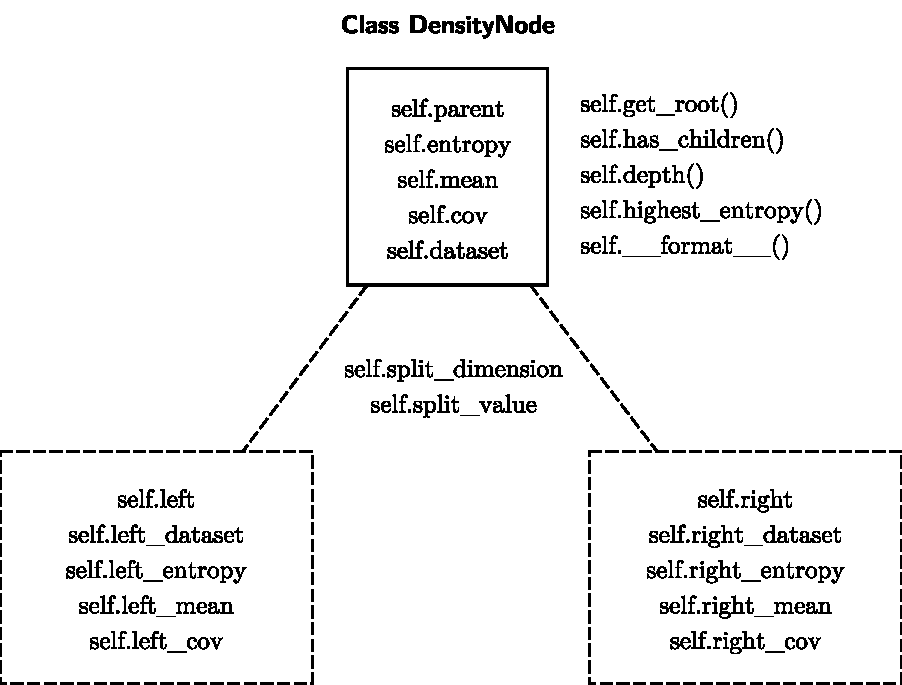
\includegraphics[width=.5\textwidth]{density-node.pdf}
    \caption{Implemented data structure for density tree nodes. Every node saves a pointer to its parent, the gaussian entropy at its level, the mean and covariance of the sub-dataset, the sub-dataset itself as well as the split dimension and split value. In addition, every node saves information about its child nodes as well as some traversal and formatting functions.}
    \label{fig:density-node}
\end{figure}



\end{document}